\documentclass[tikz,border=12pt]{standalone}
\usetikzlibrary{calc}
\definecolor{pink}{HTML}{F72585}\definecolor{blue}{HTML}{228BE6}
\definecolor{violet}{HTML}{7950F2}\definecolor{ink}{HTML}{343A40}\definecolor{soft}{HTML}{F8F9FA}
\begin{document}
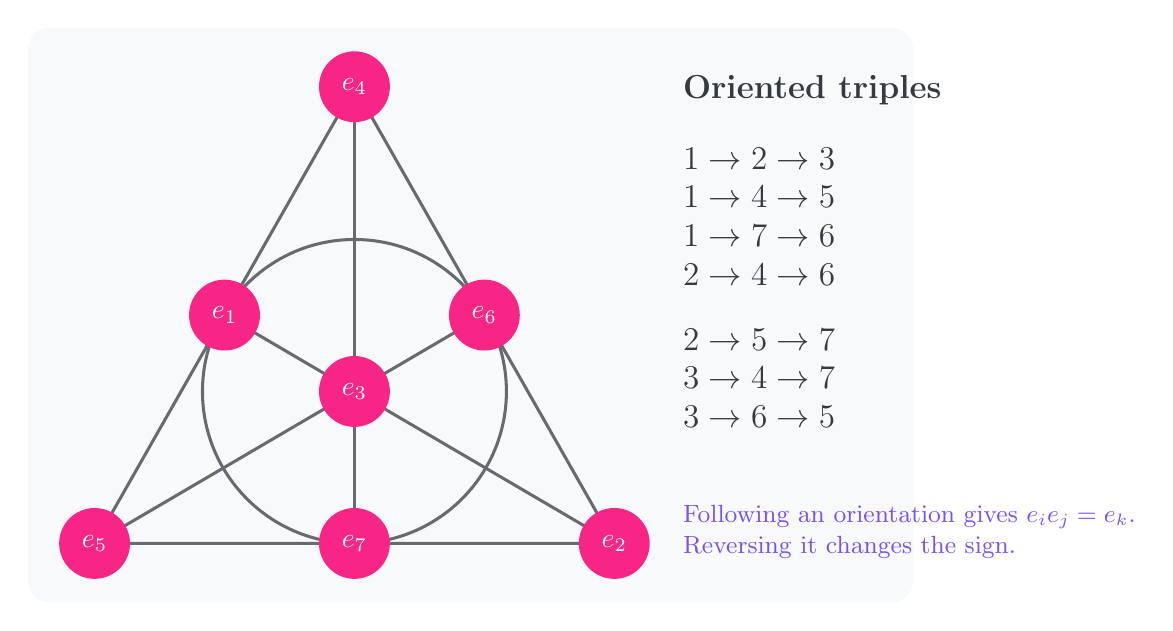
\begin{tikzpicture}[point/.style={circle,fill=pink,text=white,minimum size=9mm,font=\bfseries},line/.style={ink!75,line width=1.1pt}]
 \coordinate (p4) at (0,3.8); \coordinate (p5) at (-3.3,-2); \coordinate (p2) at (3.3,-2);
 \coordinate (p1) at ($(p4)!.5!(p5)$); \coordinate (p6) at ($(p4)!.5!(p2)$);
 \coordinate (p7) at ($(p5)!.5!(p2)$); \coordinate (p3) at (0,-.07);
 \fill[soft,rounded corners=8pt] (-4.15,-2.75) rectangle (7.1,4.55);
 \draw[line] (p4)--(p5)--(p2)--cycle;
 \draw[line] (p1)--(p2); \draw[line] (p4)--(p7); \draw[line] (p5)--(p6);
 \draw[line] (0,-.07) circle (1.93cm);
 \foreach \n in {1,...,7}{\node[point] at (p\n) {$e_\n$};}
 \node[anchor=west,font=\bfseries\large,text=ink] at (4.05,3.75) {Oriented triples};
 \node[anchor=north west,align=left,font=\large,text=ink] at (4.05,3.15)
  {$1\to2\to3$\\$1\to4\to5$\\$1\to7\to6$\\$2\to4\to6$};
 \node[anchor=north west,align=left,font=\large,text=ink] at (4.05,.85)
  {$2\to5\to7$\\$3\to4\to7$\\$3\to6\to5$};
 \node[anchor=west,align=left,font=\small,text=violet] at (4.05,-1.85)
  {Following an orientation gives $e_i e_j=e_k$.\\Reversing it changes the sign.};
\end{tikzpicture}
\end{document}
